% !TEX root = ../main.tex
\section{Experiments} \label{sec:experiments}

In this section,
we carry out a simulation study to compare
the Bayesian coverage of credible intervals
from Gaussian approximations to two different targets.
In each simulation study,
we minimized both the reverse and the forward KL divergence
using 10,000 iterations of stochastic gradient descent
with learning rate $\propto 1/\sqrt{t}$;
the proportionality constant was fine-tuned for every experiment.
The code to reproduce our experiments is available at .


\subsection{Cauchy} \label{subsec:cauchy}

First we consider approximating a Cauchy distribution
$\pi(x)=(\pi(1+x^2))^{-1}$.
This example was chosen because it gives us access to exact
credible intervals and also because of its heavy tails,
which should encourage the reverse KL-optimal
approximation to severly underestimate the variance
and viceversa with the forward KL-optimal approximation.
This is seen in \cref{fig:cauchy_lp},
where the tails of $q_\mathrm{fwd}$ are a better
approximation to those of $\pi$.
\cref{fig:cauchy_lims,fig:cauchy_coverage}
show the limits and resulting coverage of each approximation.
As expected, the $q_\mathrm{fwd}$ tends to have better coverage,
especially for large credibility values.
Specifically, for $\alpha=0.05$
the coverage is nearly exact.
On the other hand, $q_\mathrm{rev}$ produces
intervals with consistently low coverage.

\begin{figure}[ht]
    \begin{subfigure}{\linewidth}
    \centering
    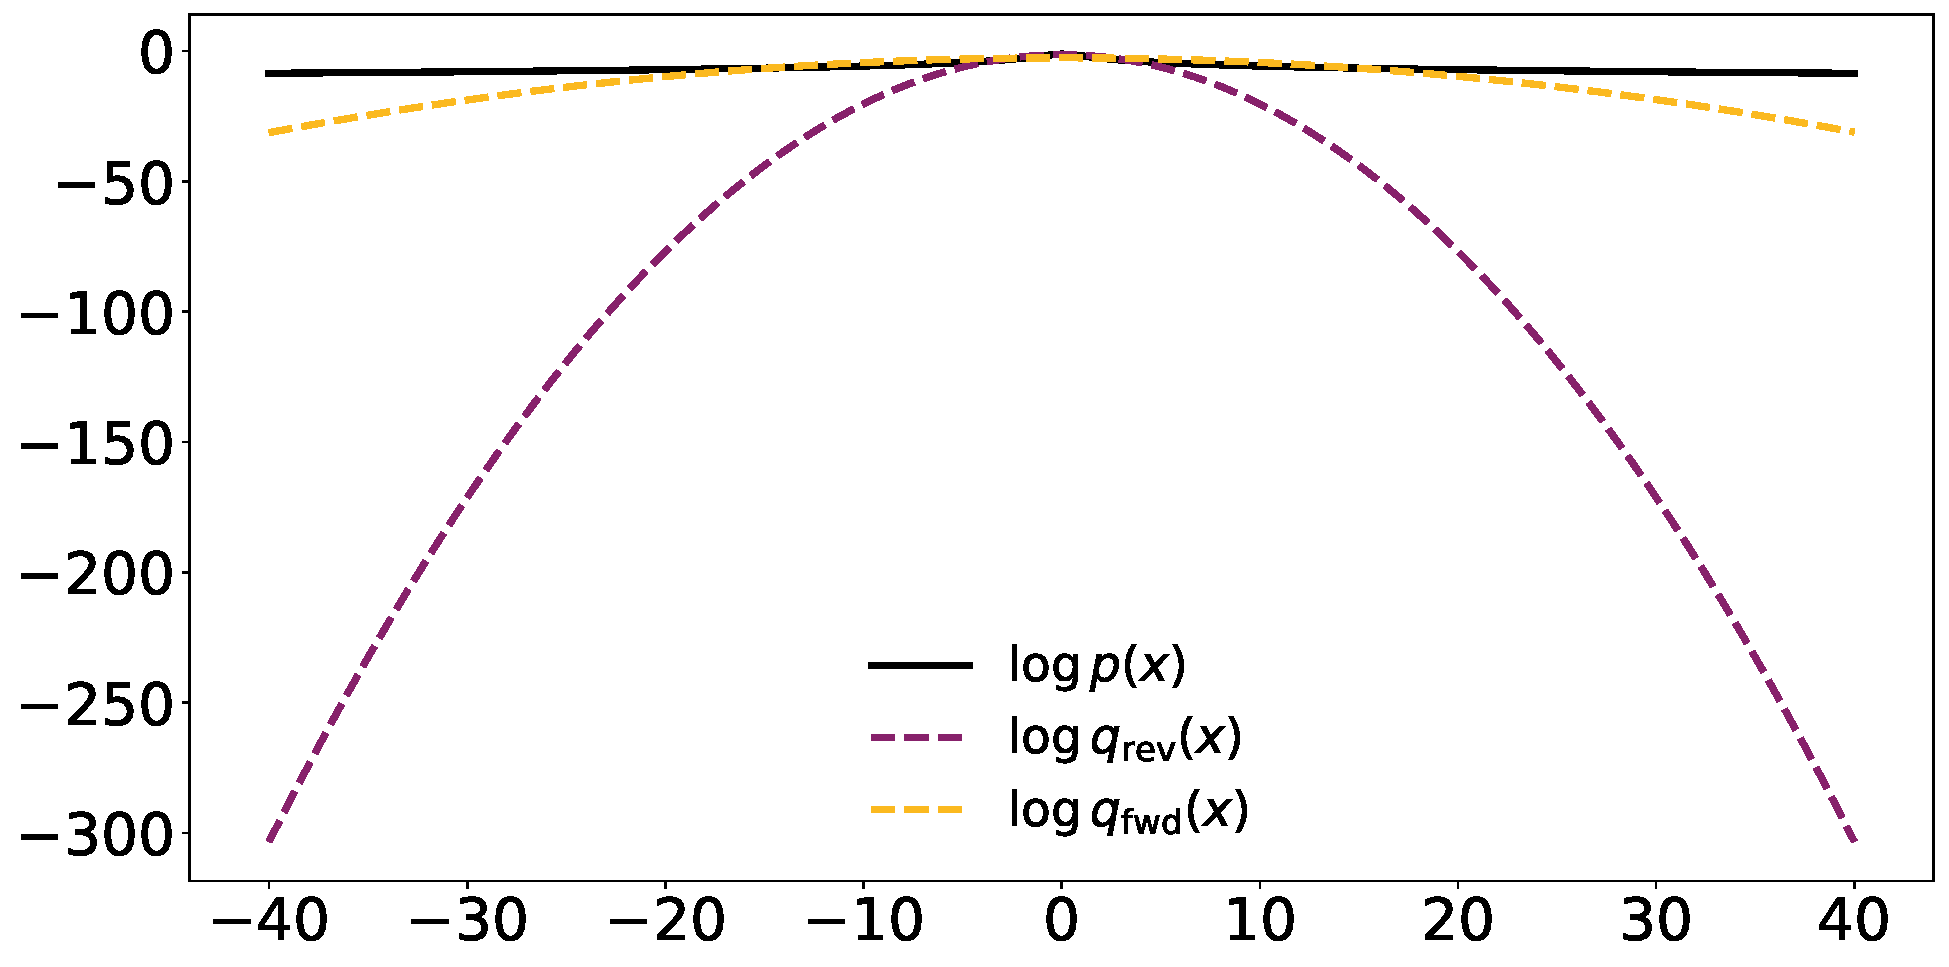
\includegraphics[width=0.8\linewidth]{fig/cauchy_logq.pdf}
    \caption{Log density}
    \label{fig:cauchy_lp}
    \end{subfigure}\\[1ex]
    \begin{subfigure}{\linewidth}
    \centering
    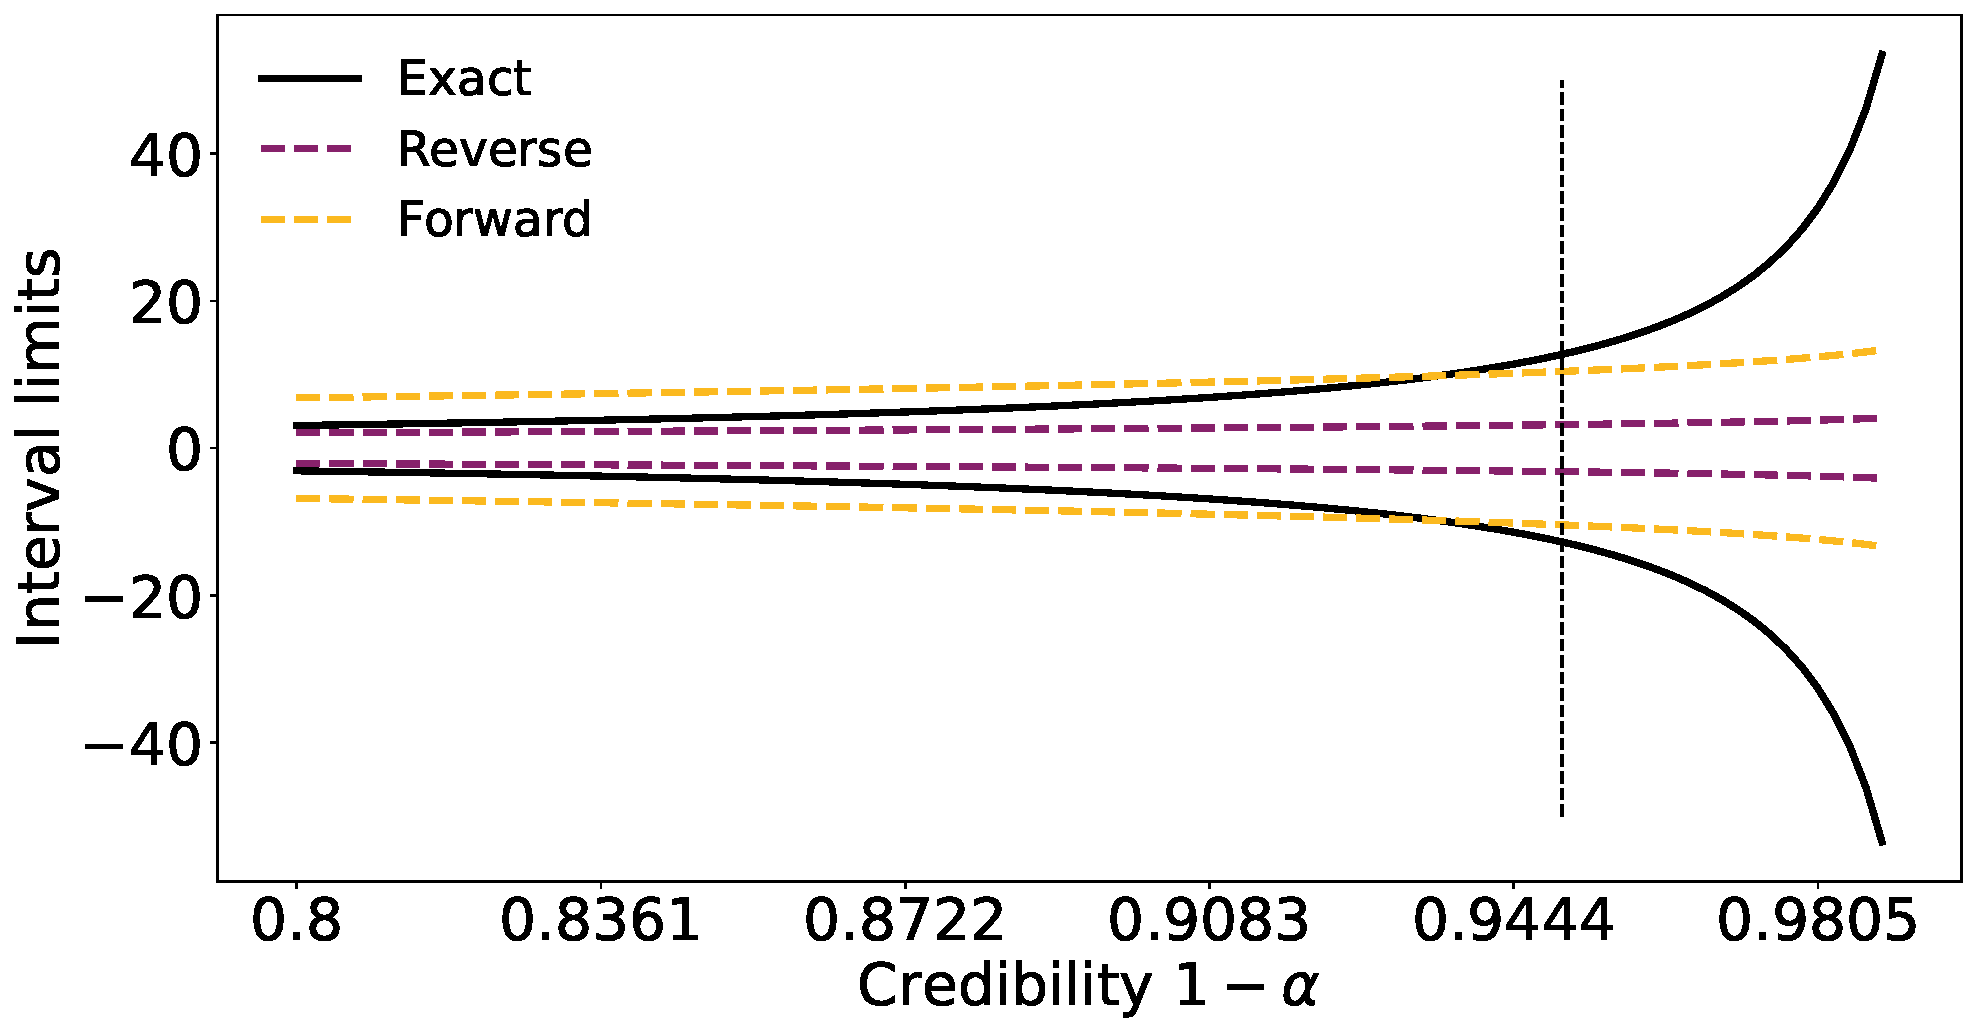
\includegraphics[width=0.8\linewidth]{fig/cauchy_cilims.pdf}
    \caption{CI limits}
    \label{fig:cauchy_lims}
    \end{subfigure}\\[1ex]
    \begin{subfigure}{\linewidth}
    \centering
    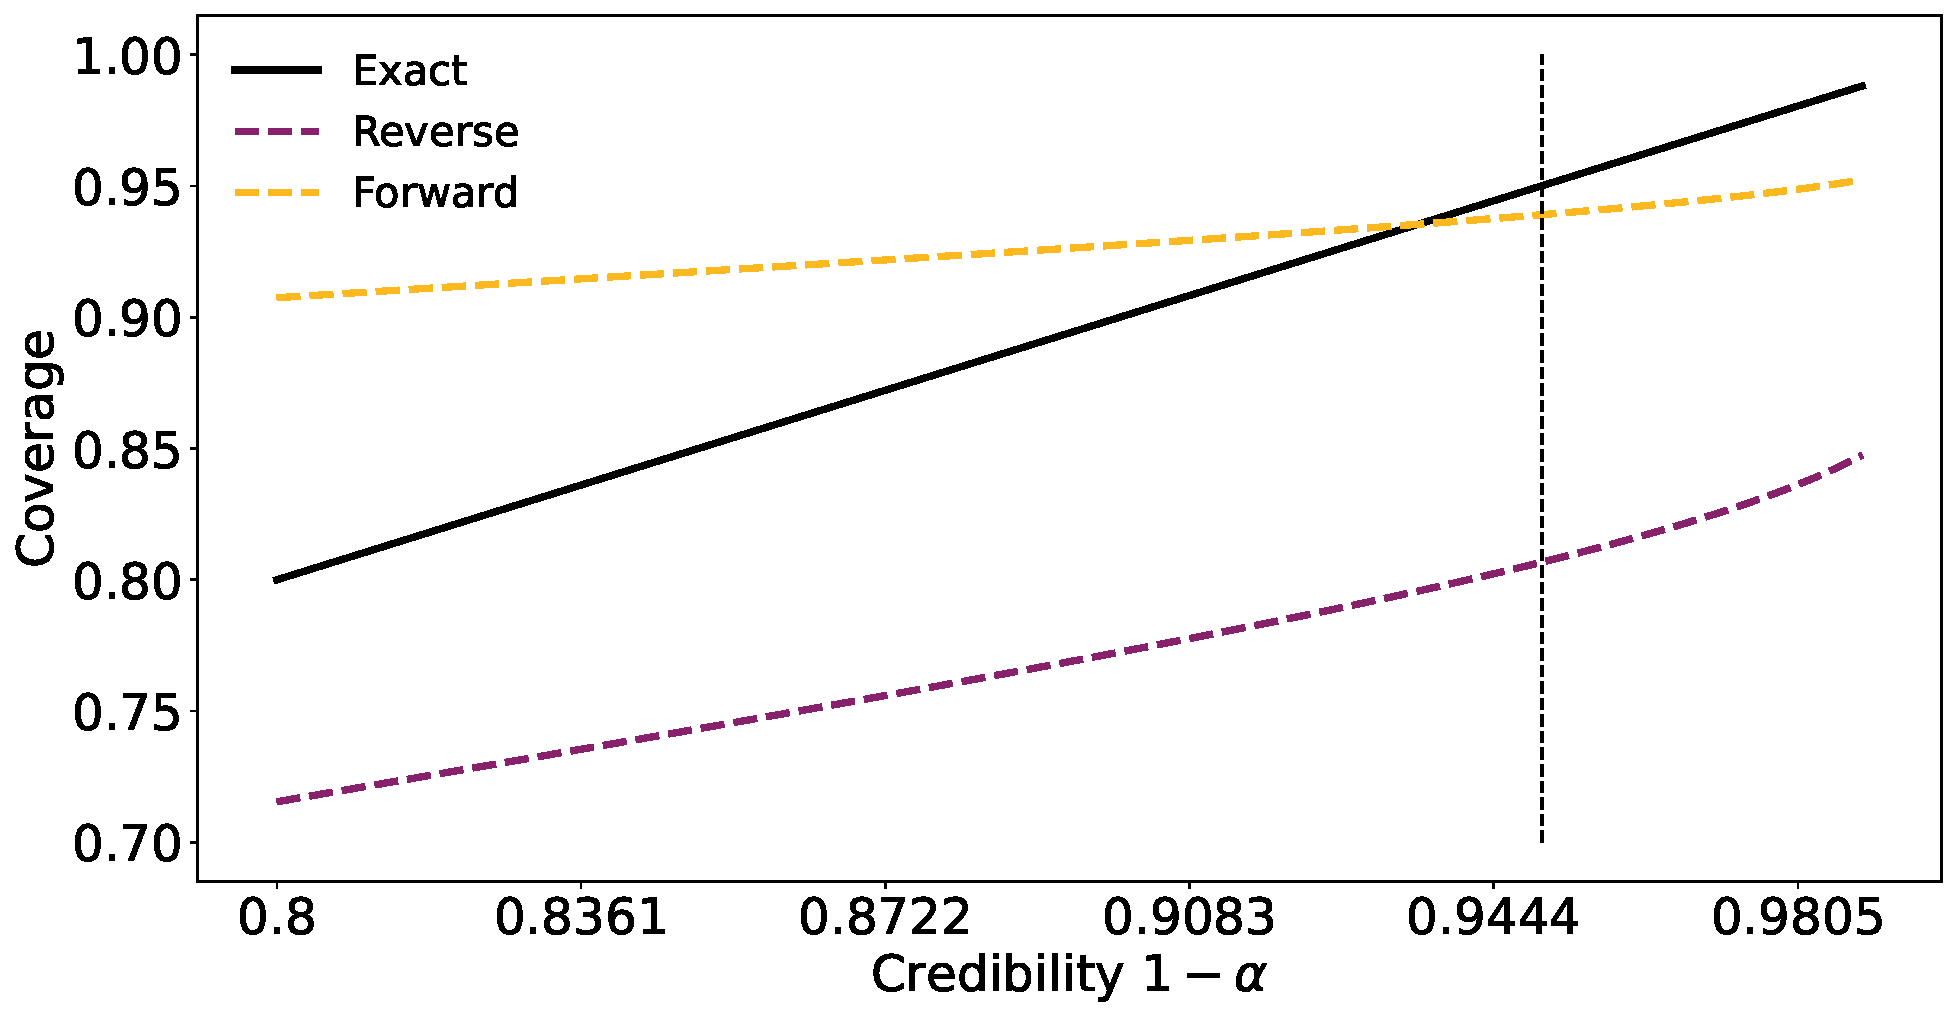
\includegraphics[width=0.8\linewidth]{fig/cauchy_cicoverage.pdf}
    \caption{CI coverage}
    \label{fig:cauchy_coverage}
    \end{subfigure}
    \caption{Results on the Cauchy distribution.}
    \label{fig:cauchy}
\end{figure}



\subsection{Logistics regression} \label{subsec:logreg}

\begin{figure}[ht]
    \begin{subfigure}{0.475\linewidth}
    \centering
    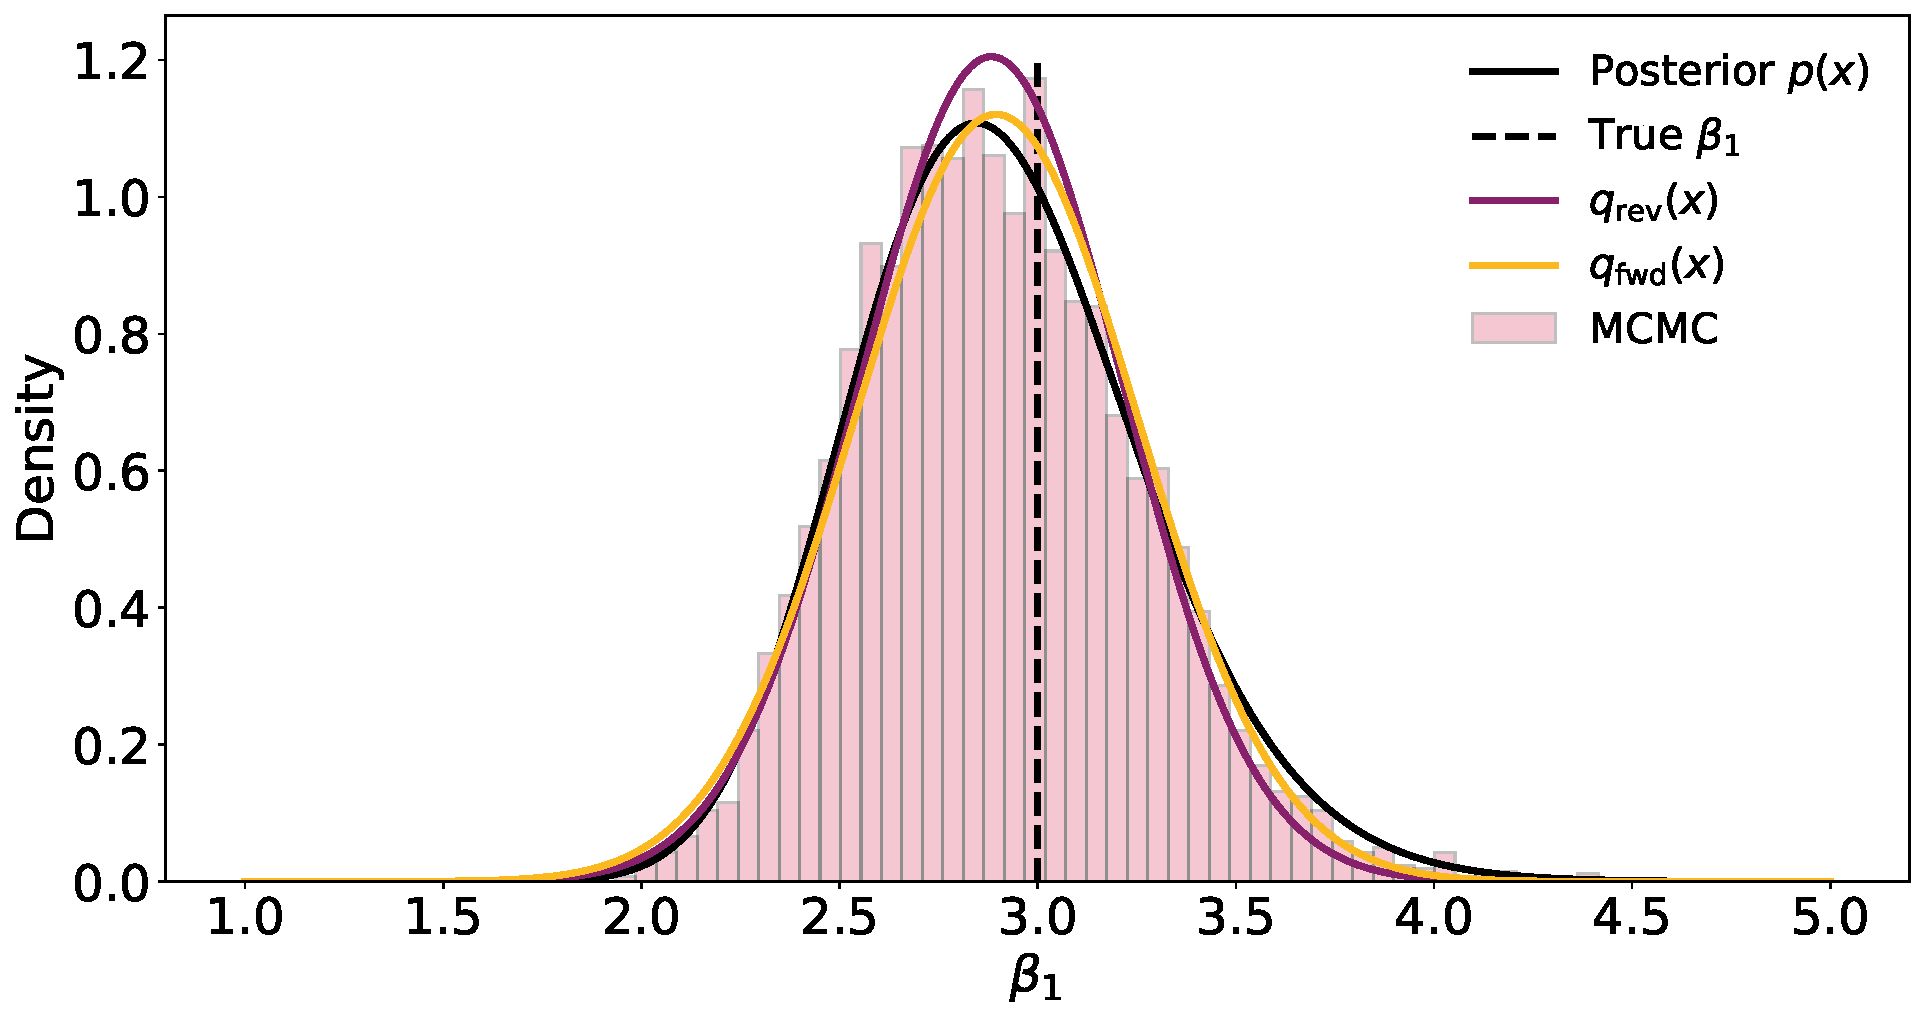
\includegraphics[width=\linewidth]{fig/logreg_q.pdf}
    \caption{Density}
    \label{fig:logreg_p}
    \end{subfigure}%
    \begin{subfigure}{0.475\linewidth}
        \centering
        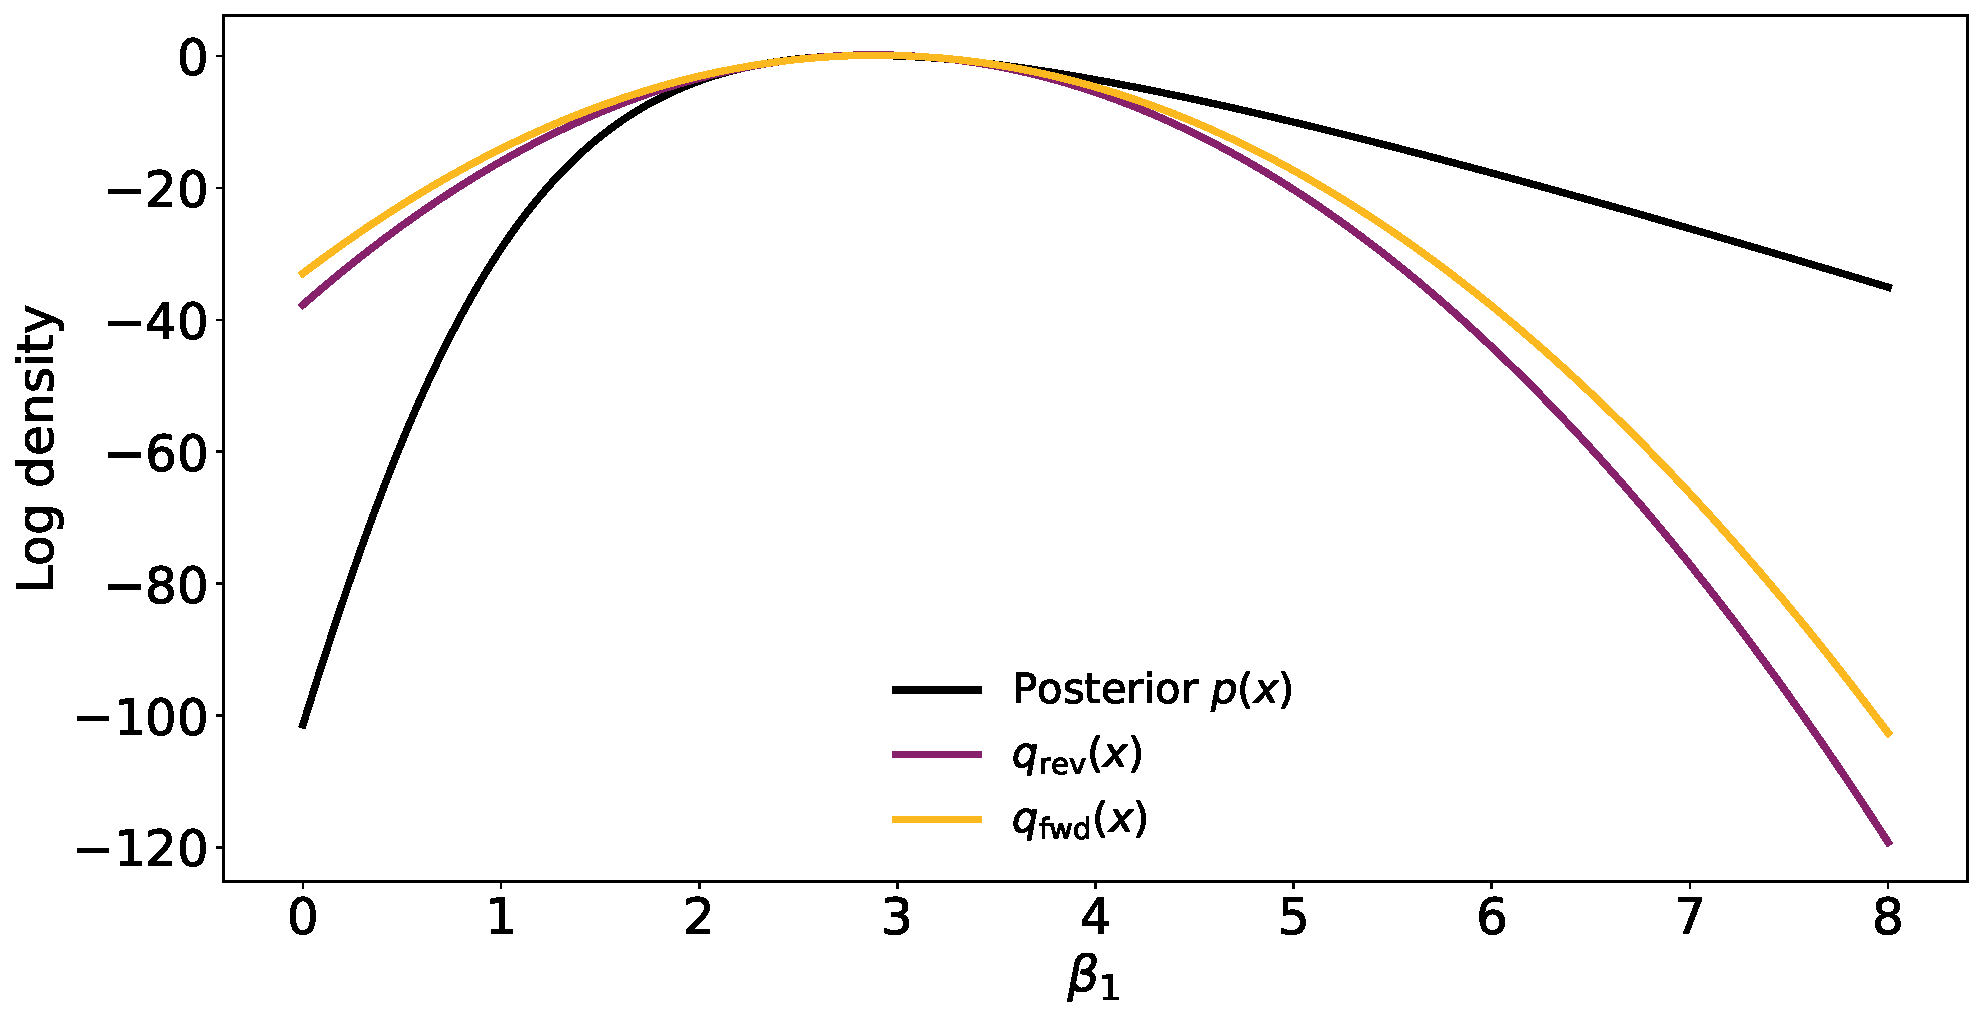
\includegraphics[width=\linewidth]{fig/logreg_logq.pdf}
        \caption{Log density}
        \label{fig:logreg_lp}
        \end{subfigure}\\[1ex]
    \begin{subfigure}{\linewidth}
    \centering
    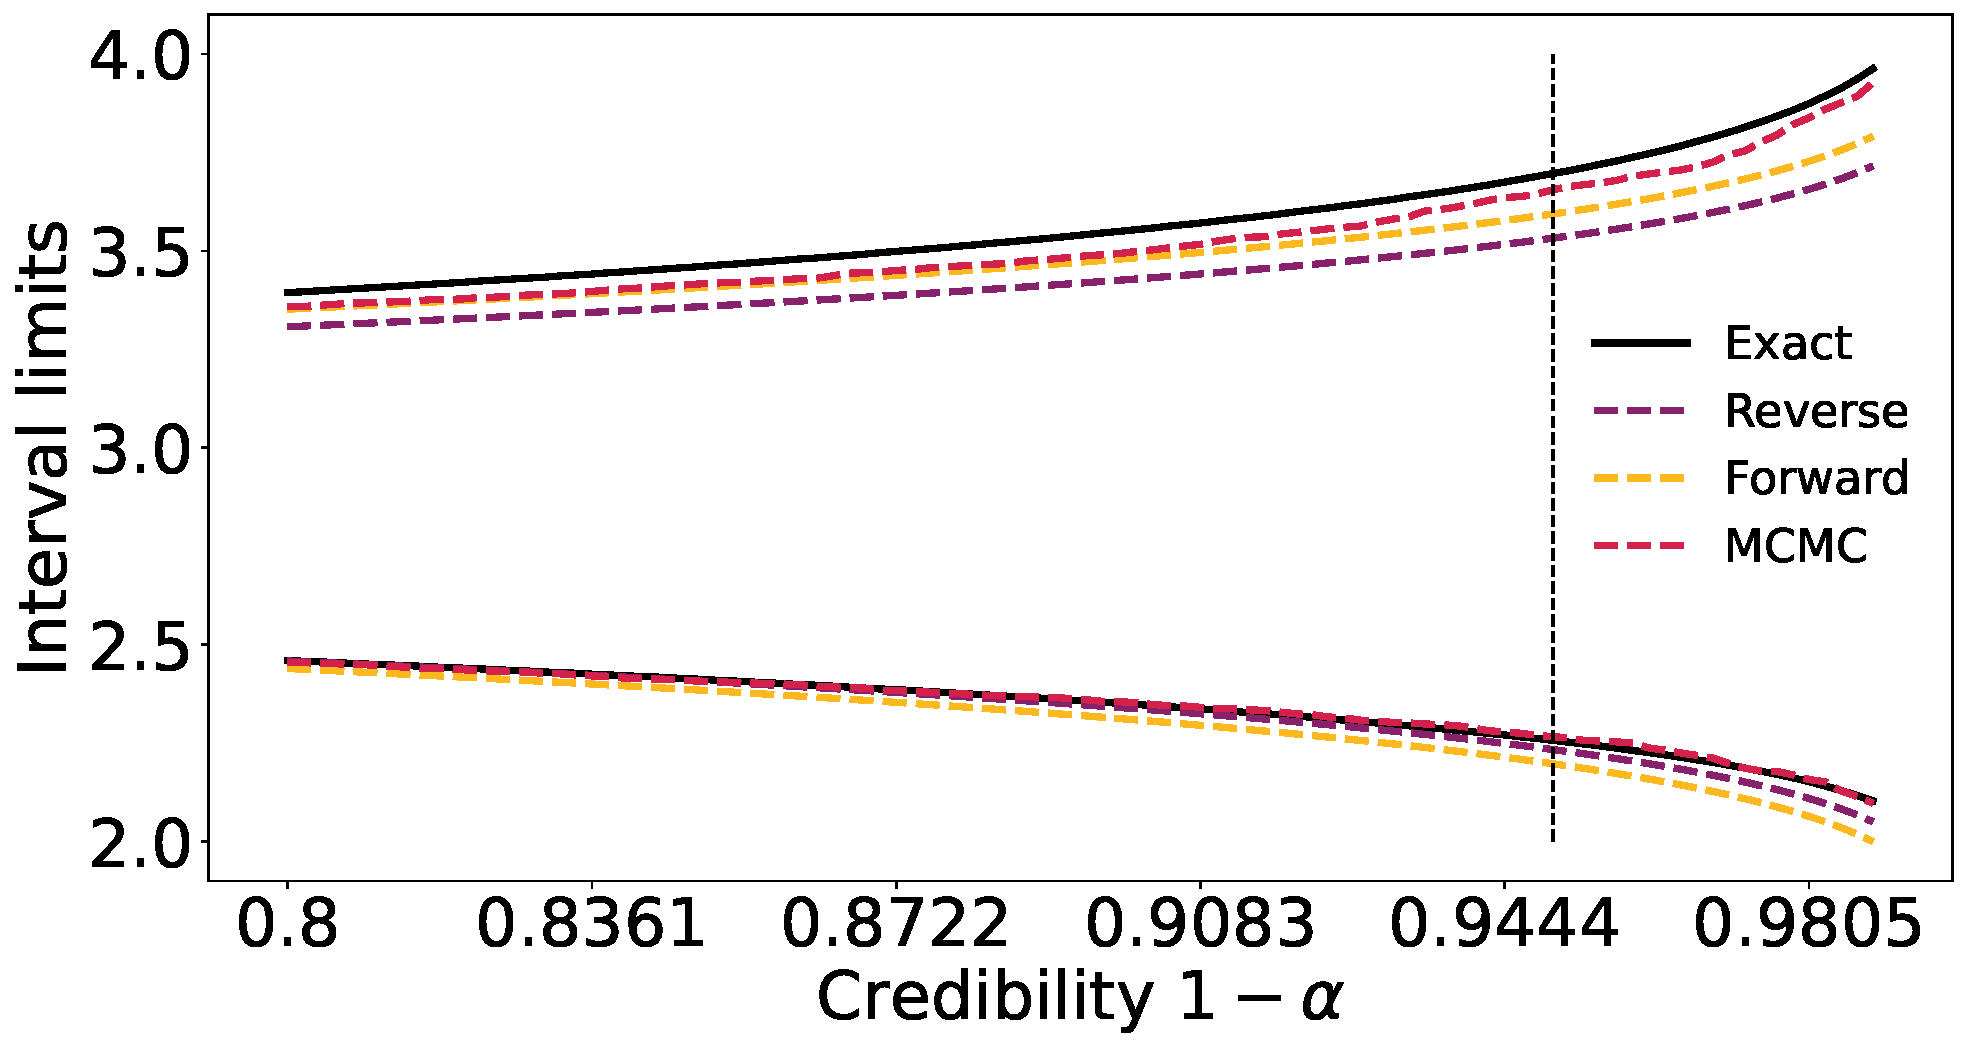
\includegraphics[width=0.8\linewidth]{fig/logreg_cilims.pdf}
    \caption{CI limits}
    \label{fig:logreg_lims}
    \end{subfigure}\\[1ex]
    \begin{subfigure}{\linewidth}
    \centering
    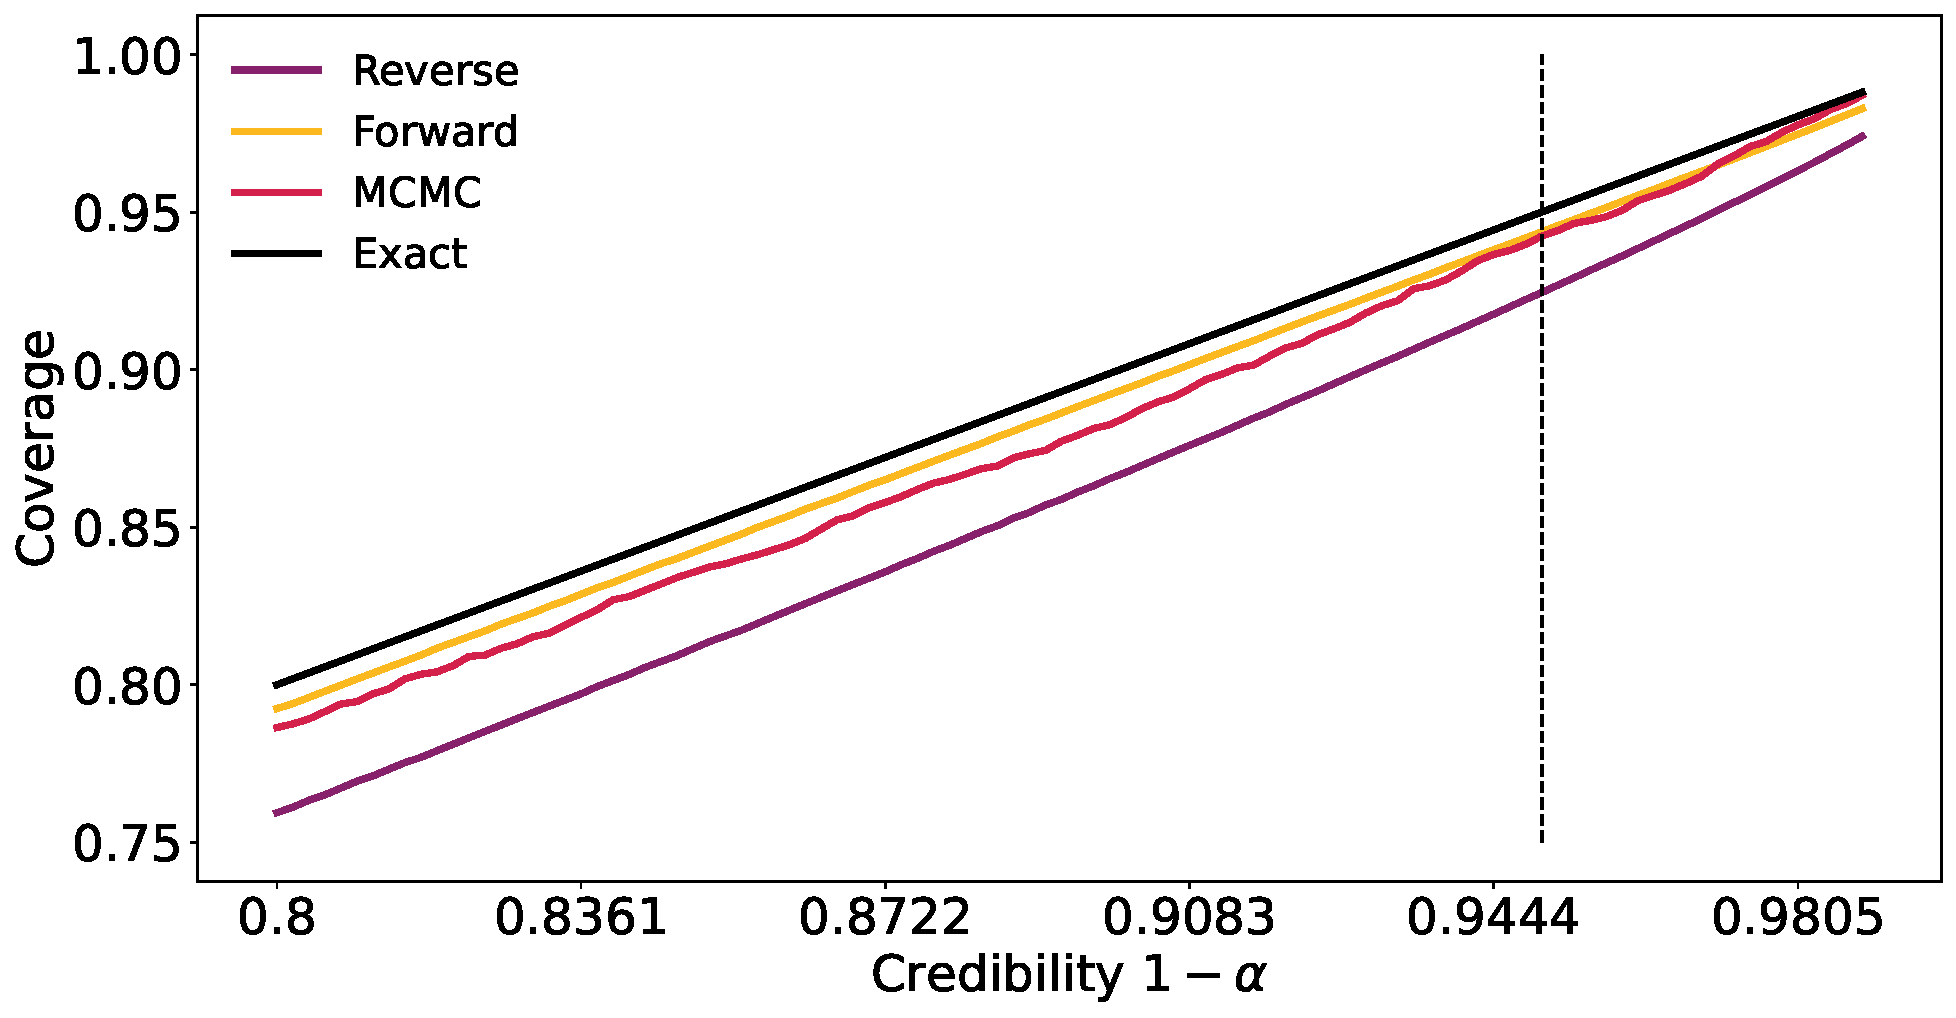
\includegraphics[width=0.8\linewidth]{fig/logreg_cicoverage.pdf}
    \caption{CI coverage}
    \label{fig:logreg_coverage}
    \end{subfigure}
    \caption{Results on the logistic regression example.}
    \label{fig:logreg}
\end{figure}
